\documentclass[12pt, twoside]{article}
\usepackage[letterpaper, margin=1in, headsep=0.5in]{geometry}
\usepackage[english]{babel}
\usepackage[utf8]{inputenc}
\usepackage{amsmath}
\usepackage{amsfonts}
\usepackage{amssymb}
\usepackage{tikz}
\usetikzlibrary{quotes, angles}
\usepackage{graphicx}
%\usepackage{pgfplots}
%\pgfplotsset{width=10cm,compat=1.9}
%\usepgfplotslibrary{statistics}
%\usepackage{pgfplotstable}
%\usepackage{tkz-fct}
%\usepackage{venndiagram}
\usepackage{multicol}


\usepackage{fancyhdr}
\pagestyle{fancy}
\fancyhf{}
\fancyhead[RE]{\thepage}
\fancyhead[RO]{\thepage \\Name: \hspace{1.5in}.\\}
\fancyhead[LO]{BECA / Dr. Huson / Geometry 10th Grade\\* Unit 9: Congruence transformations \\ 26 February 2020}

\renewcommand{\headrulewidth}{0pt}

\begin{document}
\subsubsection*{9.3 Homework: Transformation practice}
  \begin{enumerate}

  \item Given $\triangle ABC$ and $\triangle DEF$ with $\angle A \cong \angle D$ and $\angle C \cong \angle F$. What congruence is required to prove the triangles congruent using ASA? \vspace{3cm}
  
  \item Given $\triangle ABC$ and $\triangle DEF$ with $\overline{AB} \cong \overline{DE}$ and $\angle B \cong \angle E$. What congruence is required to prove the triangles congruent using SAS? \vspace{3cm}
  
  \item Given $\triangle ABC$ and $\triangle DEF$ with $\overline{AB} \cong \overline{DE}$ and $\angle A \cong \angle D$. What congruence is required to prove the triangles congruent using ASA? \vspace{3cm}
  
  \item Apply the translation $(x,y) \rightarrow (x-2,y+4)$ to the point $A(2,-1)$. \vspace{2cm}
  \item What is the image of $B(2,7)$ under a reflection across the $x$-axis? \vspace{2cm}
  \item State the translation that would map $C(-3,1)$ onto $C'(4,0)$. \vspace{3cm}

  \newpage
    \item A translation maps $D(1,9) \rightarrow D'(4,3)$. What is the image of $E(6,-2)$ under the same translation?  \vspace{3cm}

  \item The image of triangle $ABC$ after a translation is $\triangle A'B'C'$. Is the area of the triangle greater, smaller, or the same after the translation? Justify your answer. \vspace{3cm}

  \item On the graph below, draw $\overline{AB}$, with $A(-2,1)$ and $B(6,3)$, labeling the end points. Determine and state the coordinates of the midpoint $M$ of $\overline{AB}$ and mark and label it on the graph.\\
      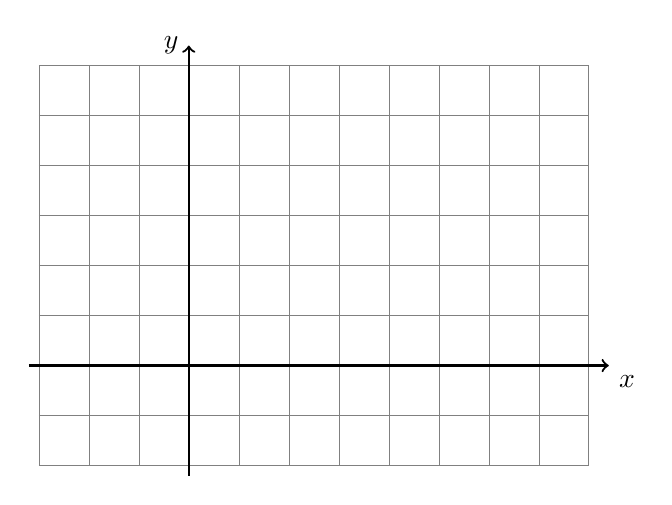
\begin{tikzpicture}[scale=.635]
        \draw [help lines] (-3,-2) grid (8,6);
        \draw [thick, ->] (-3.2,0) -- (8.4,0) node [below right] {$x$};
        \draw [thick, ->] (0,-2.2)--(0,6.4) node [left] {$y$};
      \end{tikzpicture}
      \vspace{2cm}

  \item $A(3,1)$ is one endpoint of $\overline{AB}$. The segment's midpoint is $M(7,6)$. Find the other endpoint, $B$. 
  
\end{enumerate}
\end{document}
